\section{Introduktion til mapping}
Behovet for at fremskaffe et kort over en robots omgivelser vil i den ene eller anden forstand altid være påkrævet før robotten er i stand til at interagere med det miljø den er placeret i.
Det kan f.eks. være et stort udendørs areal man ønsker at bygge et kort over, eller f.eks. robottens eget syn på den verden hvori den bevæger sig.

Der findes flere afprøvede metoder indenfor robotteknik der gør det muligt for en robot at navigere og bygge kort over dens umiddelbare nærmeste omgivelser.
Dette afsnit vil fokusere på to af disse, navnligt \textit{Occupancy Grid} og \textit{Particle Filters}, og give en overordnet beskrivelse der skal danne grundlag for valget af metode for den fortløbende udvikling af projektet.
Afslutningsvis vil de to metoder blive sammenlignet for at belyse eventuelle fordele og ulemper ved begge.

\section{Notation}
Da det er ønskværdigt at kunne give en præcis beskrivelse af robottens positur dvs. dens position og retning, vil dette afsnit kort introducere den nødvendige notation, som foreslået af \citet[s.~16-21]{probabilisticRobotics}.

\begin{itemize}
\item \textbf{Tilstand} betegner den tilstand miljøet er i; altså, robottens positur, omkringliggende objekter som vægge, bygninger osv.. 
Tilstand kan være \textit{dynamisk} (tilstanden kan ændre sig -- position af en person) og \textit{statisk} (tilstanden ændrer sig ikke -- position af en bygning).
Tilstand beskrives af variablen $x$, som også indeholder information omkring robotten selv, f.eks. dens \textit{positur}, \textit{hastighed} og dens \textit{sensorer}.

\item \textbf{Tilstand i tiden} $\mathbf{t}$ betegnes af variablen $x_t$ og beskriver den seneste \textit{kendte} tilstand. 
Den forrige seneste måling angives med $x_{t-1}$ og målingen efter den seneste som $x_{t+1}$.

\item \textbf{Målingsdata} indeholder information om robottens omgivelser til et bestemt tidspunkt. 
$z_t$ er således målingsdata til tiden \textit{t}. 
Notationen

$z_{t_1:t_2} = z_{t_1}, z_{t_1}+1, z_{t_1}+2, \dots , z_{t_2}$

betegner alle målinger fra tiden \textit{$ t_1 $} til tiden \textit{$ t_2 $}
\item \textbf{Kontrol data} indeholder information om ændring af robottens tilstand. 
Kontrol data kan for eksempel være robottens hastighed, eller en aflæsning af en motors odometer der fortæller hvor mange omdrejninger hjulet har foretaget.
$u_t$ betegner ændringen af robottens tilstand i intervallet fra \textit{t-1} til \textit{t}.
Igen betegner notation

$u_{t_1:t_2} = u_{t_1}, u_{t_1}+1, u_{t_1}+2, \dots , u_{t_2}$

mængden af kontrol data fra \textit{$ t_1 $} til \textit{$ t_2 $}.
\end{itemize}


\section{Occupancy Grids}
Disse er en familie af algoritmer som gør det muligt at generere konsistente kort ud fra målinger med usikkerhed og støj (upræcise sensor målinger).
Da et \textit{occupancy grid map} går ud fra at robottens positur er kendt, kan disse med fordel overvejes til projektet, da dens lokation bestemmes eksternt via et kamera. \cite[s.~224]{probabilisticRobotics}

\subsection{Overblik}
Den overordnede idé bag et occupancy grid er at lave en ensartet inddeling af sit kort, hvor hver enkelt celle er repræsenteret af en binær tilfældig variabel der fortæller om den pågældende celle er 'optaget' eller ej, hvor optaget betegnes som sandsynligheden $\mathcal{P}(occupied) = 1$.
Til at begynde med initialiseres hver enkelt celle med værdien $\mathcal{P}(occupied) = 0,5$ som en indikation på den aktuelle tilstand endnu ikke er kendt.
En 'ledig' celle har således værdien $\mathcal{P}(occupied) = 0$.

En simpel illustration af et occupancy grid map for det kørselsmiljø der er opstillet for vores robot kan ses på \cref{map:approx_occupancy_grid}.

\begin{figure}[h] % Kørselsmiljø og et occupancy grid
\centering
	\begin{subfigure}[b]{.45\textwidth}
	\centering
	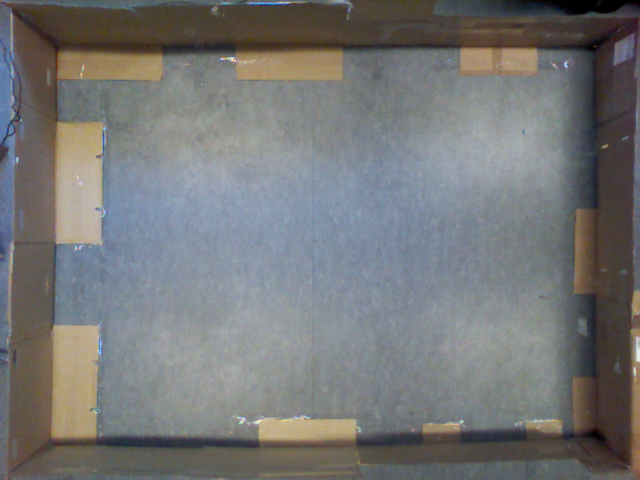
\includegraphics[width=\textwidth]{verden/oppefra}
	\caption{Aktuelt Kørselsmiljø}
	\label{map:world}
	\end{subfigure}
	\begin{subfigure}[b]{.45\textwidth}
	\centering
	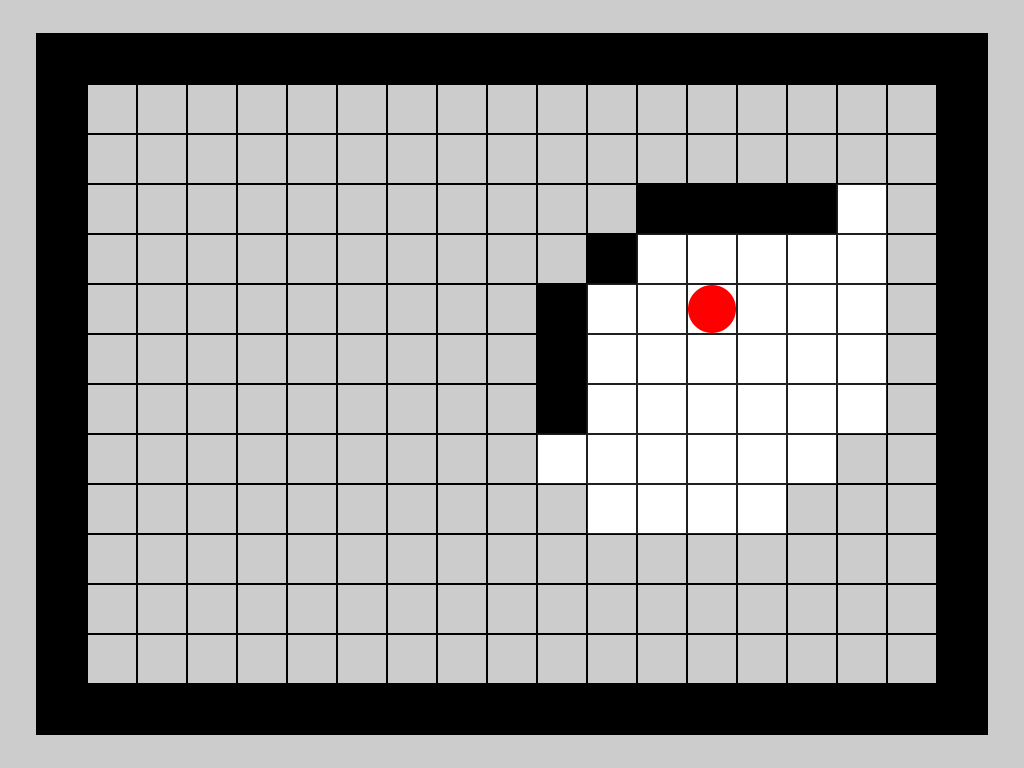
\includegraphics[width=\textwidth]{verden/occupancy_grid_verden}
	\caption{Eksempel på Occupancy Grid}
	\label{map:occupancy_grid}
	\end{subfigure}
\caption{Illustration af et occupancy grid baseret på projekts kørselsmiljø for robotten. Sorte celler i \cref{map:occupancy_grid} indikerer at $\mathcal{P}(occupied) = 1$, hvilket betegner væggene i kørselsmiljøet (\cref{map:world}). Hvide celler indikerer at $\mathcal{P}(occupied) = 0$ og grå celler angiver ikke-udforsket område. Den røde cirkel indikerer robottens position.}
\label{map:approx_occupancy_grid}
\end{figure}

\subsection{Occupancy Grid Mapping algoritme}
Den primære grund til at benytte en occupancy grid algoritme er ønsket om at få et estimat af et kort baseret på nogle antagelser om tilstanden af det omkringliggende miljø. Altså,
\\\\
\begin{equation}
\mathcal{P}(m \; | \; z_{1:t}, x_{1:t})
\end{equation}
\\\\
Hvor $m$ angiver kortet, $z_{1:t}$ mængden af alle målinger indtil tiden $t$ og $x_{1:t}$ angiver mængden af positurer for robotten (mængden af positurer over stien den har kørt).
Viden om robottens kontrol data(essentielt dens fysiske position i kortet) $u_{1:t}$, spiller her ingen rolle, da den i forvejen er kendt via Kinecten.\cite{probabilisticRobotics}

På \cref{map:occupancy_grid} gives et eksempel på en inddeling af et kørselsmiljø i $x \times y$ celler, hvor hvert enkelt celle findes ud fra et indeks $i$, således alle celler (hele kortet) beskrives ved
\\\\
\begin{equation}\label{map:occupancy_grid_sum}
m = \sum\limits_{i} \mathbf{m}_{i}
\end{equation}
\\\\
I \cref{map:occupancy_grid_sum} har hver $\mathbf{m}_i$ en værdi som beskriver om cellen er fri eller ej.
Herefter vil $\mathcal{P}(occupied) = 0$ således blive beskrevet som $\mathcal{P}(\mathbf{m}i) = 0$, for at kunne beskrive den enkelte celle.
\thilemann{Ved ikke om det er tilstrækkelig beskrivelse for at kunne sammenligne occupancy grid med particle filters og om der evt. skal indføres mere notation og måske selve occupancy grid algoritmen som angivet i \citet{probabilisticRobotics} kapitel 9.2}

\section{Particle Filters}

\section{Sammenligning}

\section{Sensor Models}

\subsection{Inverse Sensor Model}

\subsection{Forward Sensor Model	}

\